\documentclass[a4paper]{article}
% Some basic packages
\usepackage[utf8]{inputenc}
\usepackage[T1]{fontenc}
\usepackage{textcomp}
\usepackage[dutch]{babel}
\usepackage{url}
\usepackage{graphicx}
\usepackage{float}
\usepackage{booktabs}
\usepackage{enumitem}

\pdfminorversion=7

% Don't indent paragraphs, leave some space between them
\usepackage{parskip}

% Hide page number when page is empty
\usepackage{emptypage}
\usepackage{subcaption}
\usepackage{multicol}
\usepackage{xcolor}

% Other font I sometimes use.
% \usepackage{cmbright}

% Math stuff
\usepackage{amsmath, amsfonts, mathtools, amsthm, amssymb}
% Fancy script capitals
\usepackage{mathrsfs}
\usepackage{cancel}
% Bold math
\usepackage{bm}
% Some shortcuts
\newcommand\N{\ensuremath{\mathbb{N}}}
\newcommand\R{\ensuremath{\mathbb{R}}}
\newcommand\Z{\ensuremath{\mathbb{Z}}}
\renewcommand\O{\ensuremath{\emptyset}}
\newcommand\Q{\ensuremath{\mathbb{Q}}}
\newcommand\C{\ensuremath{\mathbb{C}}}

% Easily typeset systems of equations (French package)
\usepackage{systeme}

% Put x \to \infty below \lim
\let\svlim\lim\def\lim{\svlim\limits}

%Make implies and impliedby shorter
\let\implies\Rightarrow
\let\impliedby\Leftarrow
\let\iff\Leftrightarrow
\let\epsilon\varepsilon

% Add \contra symbol to denote contradiction
\usepackage{stmaryrd} % for \lightning
\newcommand\contra{\scalebox{1.5}{$\lightning$}}

% \let\phi\varphi

% Command for short corrections
% Usage: 1+1=\correct{3}{2}

\definecolor{correct}{HTML}{009900}
\newcommand\correct[2]{\ensuremath{\:}{\color{red}{#1}}\ensuremath{\to }{\color{correct}{#2}}\ensuremath{\:}}
\newcommand\green[1]{{\color{correct}{#1}}}

% horizontal rule
\newcommand\hr{
    \noindent\rule[0.5ex]{\linewidth}{0.5pt}
}

% hide parts
\newcommand\hide[1]{}

% si unitx
\usepackage{siunitx}
\sisetup{locale = FR}

% Environments
\makeatother
% For box around Definition, Theorem, \ldots
\usepackage{mdframed}
\mdfsetup{skipabove=1em,skipbelow=0em}
\theoremstyle{definition}
\newmdtheoremenv[nobreak=true]{definitie}{Definitie}
\newmdtheoremenv[nobreak=true]{eigenschap}{Eigenschap}
\newmdtheoremenv[nobreak=true]{gevolg}{Gevolg}
\newmdtheoremenv[nobreak=true]{lemma}{Lemma}
\newmdtheoremenv[nobreak=true]{propositie}{Propositie}
\newmdtheoremenv[nobreak=true]{stelling}{Stelling}
\newmdtheoremenv[nobreak=true]{wet}{Wet}
\newmdtheoremenv[nobreak=true]{postulaat}{Postulaat}
\newmdtheoremenv{conclusie}{Conclusie}
\newmdtheoremenv{toemaatje}{Toemaatje}
\newmdtheoremenv{vermoeden}{Vermoeden}
\newtheorem*{herhaling}{Herhaling}
\newtheorem*{intermezzo}{Intermezzo}
\newtheorem*{notatie}{Notatie}
\newtheorem*{observatie}{Observatie}
\newtheorem*{oef}{Oefening}
\newtheorem*{opmerking}{Opmerking}
\newtheorem*{praktisch}{Praktisch}
\newtheorem*{probleem}{Probleem}
\newtheorem*{terminologie}{Terminologie}
\newtheorem*{toepassing}{Toepassing}
\newtheorem*{uovt}{UOVT}
\newtheorem*{vb}{Voorbeeld}
\newtheorem*{vraag}{Vraag}

\newmdtheoremenv[nobreak=true]{definition}{Definition}
\newtheorem*{eg}{Example}
\newtheorem*{notation}{Notation}
\newtheorem*{previouslyseen}{As previously seen}
\newtheorem*{remark}{Remark}
\newtheorem*{note}{Note}
\newtheorem*{problem}{Problem}
\newtheorem*{observe}{Observe}
\newtheorem*{property}{Property}
\newtheorem*{intuition}{Intuition}
\newmdtheoremenv[nobreak=true]{prop}{Proposition}
\newmdtheoremenv[nobreak=true]{theorem}{Theorem}
\newmdtheoremenv[nobreak=true]{corollary}{Corollary}

% End example and intermezzo environments with a small diamond (just like proof
% environments end with a small square)
\usepackage{etoolbox}
\AtEndEnvironment{vb}{\null\hfill$\diamond$}%
\AtEndEnvironment{intermezzo}{\null\hfill$\diamond$}%
% \AtEndEnvironment{opmerking}{\null\hfill$\diamond$}%

% Fix some spacing
% http://tex.stackexchange.com/questions/22119/how-can-i-change-the-spacing-before-theorems-with-amsthm
\makeatletter
\def\thm@space@setup{%
  \thm@preskip=\parskip \thm@postskip=0pt
}


% Exercise 
% Usage:
% \oefening{5}
% \suboefening{1}
% \suboefening{2}
% \suboefening{3}
% gives
% Oefening 5
%   Oefening 5.1
%   Oefening 5.2
%   Oefening 5.3
\newcommand{\oefening}[1]{%
    \def\@oefening{#1}%
    \subsection*{Oefening #1}
}

\newcommand{\suboefening}[1]{%
    \subsubsection*{Oefening \@oefening.#1}
}


% \lecture starts a new lecture (les in dutch)
%
% Usage:
% \lecture{1}{di 12 feb 2019 16:00}{Inleiding}
%
% This adds a section heading with the number / title of the lecture and a
% margin paragraph with the date.

% I use \dateparts here to hide the year (2019). This way, I can easily parse
% the date of each lecture unambiguously while still having a human-friendly
% short format printed to the pdf.

\usepackage{xifthen}
\def\testdateparts#1{\dateparts#1\relax}
\def\dateparts#1 #2 #3 #4 #5\relax{
    \marginpar{\small\textsf{\mbox{#1 #2 #3 #5}}}
}

\def\@lecture{}%
\newcommand{\lecture}[3]{
    \ifthenelse{\isempty{#3}}{%
        \def\@lecture{Lecture #1}%
    }{%
        \def\@lecture{Lecture #1: #3}%
    }%
    \subsection*{\@lecture}
    \marginpar{\small\textsf{\mbox{#2}}}
}



% These are the fancy headers
\usepackage{fancyhdr}
\pagestyle{fancy}

% LE: left even
% RO: right odd
% CE, CO: center even, center odd
% My name for when I print my lecture notes to use for an open book exam.
% \fancyhead[LE,RO]{Gilles Castel}

\fancyhead[RO,LE]{\@lecture} % Right odd,  Left even
\fancyhead[RE,LO]{}          % Right even, Left odd

\fancyfoot[RO,LE]{\thepage}  % Right odd,  Left even
\fancyfoot[RE,LO]{}          % Right even, Left odd
\fancyfoot[C]{\leftmark}     % Center

\makeatother




% Todonotes and inline notes in fancy boxes
\usepackage{todonotes}
\usepackage{tcolorbox}

% Make boxes breakable
\tcbuselibrary{breakable}

% Verbetering is correction in Dutch
% Usage: 
% \begin{verbetering}
%     Lorem ipsum dolor sit amet, consetetur sadipscing elitr, sed diam nonumy eirmod
%     tempor invidunt ut labore et dolore magna aliquyam erat, sed diam voluptua. At
%     vero eos et accusam et justo duo dolores et ea rebum. Stet clita kasd gubergren,
%     no sea takimata sanctus est Lorem ipsum dolor sit amet.
% \end{verbetering}
\newenvironment{verbetering}{\begin{tcolorbox}[
    arc=0mm,
    colback=white,
    colframe=green!60!black,
    title=Opmerking,
    fonttitle=\sffamily,
    breakable
]}{\end{tcolorbox}}

% Noot is note in Dutch. Same as 'verbetering' but color of box is different
\newenvironment{noot}[1]{\begin{tcolorbox}[
    arc=0mm,
    colback=white,
    colframe=white!60!black,
    title=#1,
    fonttitle=\sffamily,
    breakable
]}{\end{tcolorbox}}




% Figure support as explained in my blog post.
\usepackage{import}
\usepackage{xifthen}
\usepackage{pdfpages}
\usepackage{transparent}
\newcommand{\incfig}[1]{%
    \def\svgwidth{\columnwidth}
    \import{./figures/}{#1.pdf_tex}
}

% Fix some stuff
% %http://tex.stackexchange.com/questions/76273/multiple-pdfs-with-page-group-included-in-a-single-page-warning
\pdfsuppresswarningpagegroup=1

\title{\Huge{Some Class}}
\author{\huge{Daniel Yu}}
\date{September 10, 2024}

\begin{document}
\maketitle
\newpage% or \cleardoublepage
% \pdfbookmark[<level>]{<title>}{<dest>}
\tableofcontents
\pagebreak

\section{Probability Formalism}
\subsection{Definitions and Probability Measures}
\begin{remark}
  Probability is severely counterintuitive and in fact, the following formalism of the field was only defined in the 1930s despite the hundreds
  of years of history.
\end{remark}

\begin{definition}
  Given an experiment with multiple possible outcomes, we set:
  \[
    \Omega = \{\text{ set of all outcomes} \}
  .\] 
\end{definition}

\begin{remark}
  Assume $\Omega$ is at most countable. Dealing with uncountable $\Omega$ is where measure-theoretic probability comes in.
\end{remark}

\begin{definition}
  An event A is any subset of $\Omega$. $A_i \subseteq \Omega$.
\end{definition}

\begin{definition}
  A probability measure, $P$, is any function $P: \{ \text{ events } \} \to [0,1]$, such that:
  \begin{enumerate}
    \item $P[\emptyset] = 0$
    \item  $P[\Omega] = 1$
    \item If $\{A_i\}_{i=1}^\infty$ (set of different events) is an at most countable \textbf{collection of disjoint events} then, $P[\cup_{i=1}^\infty 
      A_i] = \sum_{i=1}^{\infty} P[A_i]$.
  \end{enumerate} 
\end{definition}

\begin{note}{Example 1} 
  \\
  $\Omega = \{H , T\}$ 
  \[
    \text{ set of events } = \{ \emptyset, \{H\}, \{T\}, \{H,T\} \} 
  .\] 
  from the definition of probability measure, property 3:
  \[
    P[\{H\} \cup \{T\}] = P[\{H\}] + P[\{T\}] = P[\Omega] = 1    
  .\] 
  
\end{note}

\begin{note}{Example 2}
  \[
    \Omega = \{1,2,3,4,5,6\} \text{ A six-sided die roll for example} 
  .\] 
  $A = \{ \text{ outcome is at most 2} \} = \{1,2\}$ \\
  $B = \{ \text{ outcome is at least 5} \} = \{5,6\}$
  \[
    P[A \cup B] = P[A] + P[B]
  .\] 
\end{note}

\begin{remark}
  Suppose that $P[w]$ is the same for all $w \in \Omega$. So in particular, $P[\{1\}] = \frac{1}{|\Omega|} = \frac{1}{6}$
  so for any event $A$,
  \[
    P[A] = P[\cup_{w \in A} \{w\}] = \sum_{w \in A} P[\{w\}] = \frac{|A|}{|\Omega|}  
  .\]. This simplifies to counting, very easy, but of course a measure need not be uniform \ldots
\end{remark}

\begin{note}{Example 3}
  \\
  Assume that there is a pile of cards of color, R, G or B and I drew one at random
  \[
    P(R \cup B) = \frac{3}{5}
    P(R \cup G) = \frac{3}{5}
  .\] 
  what is the probability of $P[R]$? \\
  We know that $\Omega = \{R,G,B\}$
  \[
    P[R] + P[B] + P[G] = 1
  .\] 
  \[
    P[R] + P[B] = \frac{3}{5}
  .\] 
  \[
  P[R] + P[G] = \frac{3}{5}
  .\] 
  We get $P[R] = \frac{1}{5}$. \\

  Notice that we are solving a \textbf{determined} system!
\end{note}

\textbf{Properties}\\
There are a few consequences of the definition: 
\begin{enumerate}
  \item $P[A^c] = 1 - P[A]$. \\ Proof:  $P[\Omega] = 1 = P[A \cup A^c] = P[A] + P[A^c]$
  \item If $A \subseteq B$, $P[A] \leq P[B]$.  \\ Proof: $P[B] = P[A \cup \{B \setminus A \}] = P[A] + P[B \setminus A]$. 
    We know that $P[B \setminus A] \geq 0$, so $P[B] \geq P[A]$
  \item If we have an arbitrary at most countable collection of events (not just disjoint) $\{ B_i \}_{i=1}^\infty$, then
    $P[\cup_{i=1}^\infty B_i] \leq \sum_{i=1}^\infty P[B_i]$. Intuition is that $B_i$ may overlap events(i.e. outcomes) with $B_j$ and we double count
    so it provides an upper bound.
\end{enumerate}

\begin{note}{Example 4} \\
  52 card deck, and we draw 3 cards to form a hand. If all hands have the same possibility, what is the probability of getting 
  three 2's. \\

  $\Omega = \{ \text{ of all possible 3 card combinations without concern for order } \}$. Note that it is not the set 
  of all 52 cards! 
  \[
   |\Omega| = \begin{pmatrix} 52 \\ 3 \end{pmatrix} = \frac{52 \times 51 \times 50}{6}
  .\] 
  and the associated probability measure $P[w] = \frac{1}{|\Omega|}$ for any $w \in \Omega$. 
  \[
    A = \{ \text{hands of three 2's } \} = \{ \{2Hearts, 2C, 2D \}, \{2H, 2C, 2S\}, \{2H, 2D, 2S\}, \{2C, 2D, 2S\} \}
  .\] 
  \[
  P[\text{ getting 3 2's in hand} ] = \frac{|A|}{|\Omega|} = \frac{4}{\text{52 choose 3}}
  .\] 

  If we instead, consider the outcomes as cards dealt in order (i.e. order matters), then:
  \[
  |\Omega'| = 52 \times 51 \times 50. 
  .\] 
  i.e. in this case cards are no longer unordered triplets (a set) but ordered triples! So,
  \[
    B \subseteq \Omega' = \{ \text{hand of three 2's} \} = 4 \times 3 \times 2
  .\] 
  \[
    P[\text{choose 3 2's in hand}] = \frac{24}{52 \times 51 \times 50}
  .\] 
  Note that the two approachs give the same answer!
\end{note}

\subsection{Random Variable}
Start
\begin{definition}
 A random Variable is any map from $\Omega$ to $\R$ or ($\R^n$). 
\end{definition}

\begin{note}{Example}
  $\Omega = \{ H, T\} $
   \[
     X = \{1 \text{head}, 0 \text{tail} \} 
   .\] 
  
   Suppose $P[\{H\}] = \frac{1}{3}$. Therefore,
   \[
     P[X=1] = \frac{1}{3}
   .\] 
   \[
     P[X=0] = \frac{2}{3}
   .\] 
\end{note}
\begin{definition}
  The \textbf{distribution} of $X$ is the $P[X = a]$ for every $a$ where $a \in \R$ and $a \neq 0$. 
  Note that \textbf{the distribution of a random variable is the measure it induces on $\R$}
\end{definition}

\begin{remark}
  For any set $S \subseteq \R$, at most countable, we can describe a distribution such that $P[x = a]\geq 0$ $\forall a \in S$
  and $P[x=a] = 0$ otherwise. Any function (probability measure) that satisfies:
  \begin{enumerate}
    \item $P[x=a] \geq 0$ for $a \in S$
    \item $\sum_{a \in S} P[x=a] = 1$
  \end{enumerate}
\end{remark}

\begin{remark}{Infinite Set} \\
  $\Omega = \left\{ 1,2,3, \ldots \right\}$, an infinite set. \\
  Assume that $P[z=k]$ forms a geometric series, pick $p \in (0,1]$ and set $P[z=k] = p \cdot (1-p)^{k-1}$. This is a distribution:
  \[
    p [1 + (1-p) + (1-p)^{2} + (1-p)^{3} + \ldots ] = p \cdot \frac{1}{1 - \frac{1}{p}} = 1
  .\]
  So this does form a probability distribution. Note that $p \neq 0$ because then this would go to 0. 
\end{remark}

\begin{remark}{Poisson Distribution} \\
  $R \sim \text{ Poisson}(\lambda)$ means that R is distributed as a poisson  distribution. 
   \[
     P[R = k] = \frac{e^{-\lambda} \cdot \lambda^k}{k!}   \forall   k \in \left\{ 0,1,2,3, \ldots \right\} 
  .\] 
  It turns out this is also a distribution:
  \[
  e^{- \lambda} (\sum_{k=0}^\infty \frac{\lambda^k}{k!}) = 1
  .\] 
\end{remark}


\begin{note}{Example}
  \[
    \Omega = \{1,2,3,4,5,6\}. \text{ P is uniform}.
  .\] 
  \[
    Y = \{1 \text{if w is divisible by 3} , 0 \text{if w is not} \} 
  .\] 
  The distribution of $Y$ is: 
  \[
    P[Y=1] = \frac{1}{3}
  .\] 
  \[
    P[Y=0] = \frac{2}{3}
  .\] 
  \[
    P[Y=\alpha] = 0 \forall \alpha \not\in \{0,1\} 
  .\] 
\end{note}

\begin{remark}
  Even though X and Y are different random variables, they \textbf{share the same distribution}
\end{remark}

\begin{definition}
  If \[
    P[X=1] = p
  .\] 
  \[
    P[X=0] = 1 -p
  .\] 
  We say x is distributed as a \textbf{Bernoulli random variable} of parameter $p$.
\end{definition}

\begin{note}{Example}
  \[
    \Omega = \{ \text{outcome of two rolls of a 6-sided die} \} \text{where P is uniform}
  .\] 
  $M$ is the random variable represnting the maximum of 2 rolls.
  What is the distribution of M?

  $P[M = x] = \frac{6^2 - x^2}{6^2}$
\end{note}

\subsection{CDFs and PDFs}
\begin{definition}
  Given a random variable $X$, the \textbf{cumulative distribution fuction (cdf)} of $X$, denoted as $$F_X (t) = P[X \leq t]$$.
  With the properties:
 
\begin{enumerate}
  \item $\lim_{t \to -\infty} F_x(t) = \lim_{t \to -\infty} P[x \leq t] = 0$
  \item $\lim_{t \to \infty} F_x(t) = 1$
  \item if $s \leq t$, $F_x(s) \leq F_x(t)$ i.e. it is non-decreasing 
\end{enumerate} 
\end{definition}


\begin{note}
  Thus everything we've done up to this point has been with probability measure, not cdfs, pdfs, etc. yet!
\end{note}  

\begin{note}{Bernoulli} \\
  So if $X=$ Bernoulli distribution then the cdf would be: \\
  \[
   P[x \leq -17] = 0
  .\] 
  \[
    P[x \leq 0] = P[x=0] = 1 - p 
  .\] 
  \[
    P[x \leq \frac{2}{3}] = P[x=0] = 1 -p 
  .\] 
  \[
    P[x \leq 1] = 1 
  .\] 
  \[
   P[x \leq 2] = P[x \leq 1] = 1
  .\] 
\end{note}
\begin{note}
  In general, an discrete random variable would create a piecewise cdf!
\end{note}

\begin{note}
  If we pick $U \in [0,1]$ uniformly, then $F_U (t)$ would be 0 until x = 0, then from x = 0 to x = 1, it would 
  increase along the line $y=x$, then at $x\geq1$, it would be a straight line with value $1$.
\end{note}

\begin{definition}
  The \textbf{probability density function (pdf)} of a continuous r.v. is:
  \[
  f_X\left( t \right) = \frac{d}{dt} F_X(t) 
  .\], the first derivative of the cdf. With the two properties:
  \begin{enumerate}
    \item $f_x(t) \geq 0$
    \item  $\int_{-\infty}^{\infty} f_x(t) = 1$
  \end{enumerate}
  The way to interpret $f_X \left( t \right)$ is that $X$, the random variable, is a function that maps from 
  outcomes $\Omega \to \R$ and $t$ are values $\in range(X) = \R$. So when we parameterize by $t$ we are
  letting $t$ vary across the range of values that the random variable $X$ could take. 
\end{definition}

\begin{note}
  The pdf of uniform $[0,1]$ random variable:
  \[
  f_x(t) = \begin{cases}
  \item 1, t \in [0,1] \\
  \item 0, \text{ otherwise}
  \end{cases}
  .\]   
\end{note}

\begin{prop}
  If x is a random variable and $a < b$, then
  \[
    P[ a < x \leq b] = F_x(b) - F_x(a)
  .\] 
  If the r.v. is continuous, then:
  \[
    P[ a < x \leq b] = \int_a^b f_x(t) dt
  .\] 
\end{prop}
Fundamental theorem of calc lol

\begin{proof}
  \begin{align*}
    F_x(b) - F_x(a) &= P[x \leq b] - P[x \leq a]
  .\end{align*}
  We know that by set theory
  \[
    P[ x \leq b] = P[\left\{ x \leq a \right\} \cup \left\{ a < x \leq b \right\} ] = P[x \leq a] + P[a < x \leq b]
  .\] 
  Subsitute back to equation 1.
  \[
    F_x(b) - F_x(a) =  P[x \leq a] + P[a < x \leq b] - P[x \leq a] = P[a < x \leq b] 
  .\] 
  By the fundamental theorem of calculus this holds for the continuous case: 
\end{proof}

\begin{note}
  Consider 
  \[
  f_U (t)dt = 
  \begin{cases}
  \item c, t \in [a,b] \\
  \item 0 \text{ otherwise}
  \end{cases}
  .\] 
  To find c:
  \[
    \int_{-\infty}^\infty f_U (t) dt = 1 
  .\] 
  \[
    \int_a^b cdt = = c \cdot (b - a) = 1 
  .\] 
  Thus the cdf is: 
  \[
  \begin{cases}
  \item \frac{1}{b-a}, t \in [a,b] \\
  \item 0 \text { otherwise}
  \end{cases}
  .\] 
\end{note}

\begin{note}{Exponential Distribution} \\
  $z \sim \exp(\lambda)$ of it's pdf is: \\
  \[
  f_z (t) = \begin{cases}
    \lambada e^{-\lambda t}, t \in [0, \infty] \\
    0, \text{otherwise}
  \end{cases}
  .\] 

\begin{figure}[H]
  \centering
  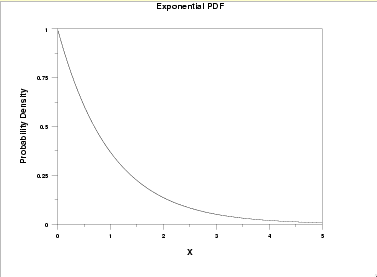
\includegraphics[width=0.8\textwidth]{assets/2024-09-12-22-08-15.png}
  \caption{Exponential Distribution PDF}
  \label{fig:2024-09-12-22-08-15}
\end{figure}
  What is it's cdf?
  \begin{align*}
    F_z(t) &= \int_{-\infty}^t f_z(s) ds =  \int_{0}^t f_z(s) ds =  \int_{0}^t \lambda e^{-\lambda s} ds  \\ 
           &= -e^{-\lambda t - (-1)} = 1 - e^{-\lambda t} 
  .\end{align*}
\end{note}

\begin{figure}[h]
  \centering
  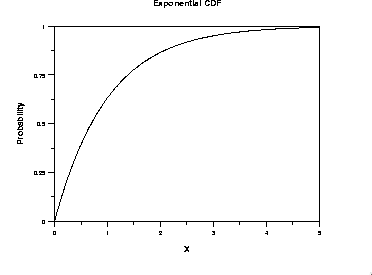
\includegraphics[width=0.8\textwidth]{assets/2024-09-12-22-14-13.png}
  \caption{Exponential Distribution CDF}
  \label{fig:2024-09-12-22-14-13}
\end{figure}

\subsubsection{Normal Distribution}
We denote the normal distribution as $N \sim \text{ normal}(\mu, \sigma^2)$. \\ 
The pdf of the normal distribution is: $f_N(t) = \frac{1}{\sigma \cdot \sqrt{2 \pi} }e^{-\frac{(t - \mu)^2}{2\sigma^2}}$

\begin{note}
  Let $X \sim N(0,1)$ and $Y = X^2$. What is the pdf of $Y$? HARD. So let's look at CDF instead:
  \begin{align*}
    F_Y(t) &= P[Y < t] = P[x^2 \leq t ] = P[- \sqrt{t} \leq x \leq \sqrt{t}] \\ 
           &= \int_{-\sqrt{t}}^{\sqrt{t}} \frac{1}{\sqrt{2\pi}} e^\frac{-x^2}{2} dx   \text{ the function is even} \\
           &= 2 \int_{0}^{\sqrt{t}} \frac{1}{\sqrt{2\pi}} e^\frac{-x^2}{2} dx 
  .\end{align*}
  Now take the pdf of $Y$ by taking first derivative w.r.t. t:
  \[
    \frac{d}{dt}\left(2 \int_0^{\sqrt{t}}  \frac{1}{\sqrt{2\pi}} e^\frac{-x^2}{2} dx  \right) 
  .\] 
  let $u = \sqrt{t}$, $\frac{d}{dt} = \frac{d}{du} \cdot \frac{du}{dt}$ :
  \[
    =\frac{d}{du}\left(2 \int_0^{u}  \frac{1}{\sqrt{2\pi}} e^\frac{-x^2}{2} dx  \right) \cdot \frac{du}{dt}
  .\] 
  \[
    = 2 \cdot \frac{1}{\sqrt{2 \pi}} \cdot e^{\frac{-\sqrt{t}^2}{2}} \cdot \frac{d(\sqrt{t})}{dt} 
  .\] 
  \[
  = \frac{1}{\sqrt{2 \pi t}} \cdot e^\frac{-t}{2}
  .\]
  This is known as the chi-squared distribution with 1 degree of freedom.
\end{note}

\section{Joint Distributions}
We need joint dsitributions to describe the behavior of multiple random variables, we need the joint distributions.
The marginal distributions are not enough! 

\begin{note}
  For example, consider the discrete random variables $x,y,z$ over $\Omega = \left\{ 1,2,3,4 \right\}$ on a uniform
  probability measure:
  \[
  X = \begin{cases}
    1, w \in \left\{ 1,2 \right\} \\
    0, w \in \left\{ 3,4 \right\} 
  \end{cases}
  .\] 
  \[
  Y = \begin{cases}
    1, w \in \left\{ 3,4 \right\} \\
    0, w \in \left\{ 1,2 \right\} 
  \end{cases}
  .\] 
  \[
  z = \begin{cases}
    1, w \in \left\{ 1,3 \right\} \\
    0, w \in \left\{ 2,4 \right\} 
  \end{cases}
  .\] 
  The marginal distribution of $X,Y,Z$ are bernoulli distributions with $p = .5$. (But they are not the same r.v.).
  Moreover, $P[X=Y]= 0$ and $P[X=Z] = .5$ despite the fact that X, Y, Z are random variables with same distribution 
  (seeming in contradiction to above)! The marginal distributions give an incomplete idea!
\end{note}

Thus we need the joint distribution! \\

If $X,Y$ are continuous random variables, we need to understand them via joint cdf or joint pdf.
\[
  F_{X,Y} = P[X \leq s, Y \leq t]
.\] 

\begin{remark}{Example}\\
  We are dealing 3 cards out of a 52 card deck with uniform probability.
  \[
  X=\begin{cases}
    1 \text{ if 1st card is ace} \\ 
    0 \text{ otherwise}
  \end{cases}
  .\] 
  \[
  Y=\begin{cases}
    1 \text{ if 2nd card is ace} \\
    0 \text{ otherwise}
  \end{cases}
  .\] 
  \[
  Z=\begin{cases}
    1 \text{ if 3rd card is ace} \\
    0 \text{ otherwise} 
  \end{cases}
  .\]
  clearly $P[X = 1] = \frac{4 \cdot 51 \cdot 50}{52 \cdot 51 \cdot 50} = \frac{1}{13}$ \\
  
  What is the joint probability distribution of $X$ and $Y$?\\
  $P[X=0, Y= 0] = \frac{48 \cdot 47 \cdot 50}{52 \cdot 51 \cdot 50}$ \\
  $P[X=0, Y =1] = \frac{48 \cdot 4 \cdot 50}{52 \cdot 51 \cdot 50}$ \\
  $P[X=1, Y=0] = \frac{4 \cdot 48 \cdot 50}{52 \cdot 51 \cdot 50}$ \\
  $P[X=1, Y=1] = \frac{4 \cdot 3 \cdot 50}{52 \cdot 51 \cdot 50}$ \\
 
  We can recover the marginal distribution of Y through this: \\
  $P[X=0, Y=0] + P[X=1, Y=0] = P[Y=0] = \frac{48\cdot 50 (4 + 47)}{52 \cdot 51 \cdot 50} = \frac{48}{52} = \frac{12}{13}$ and thus $P[Y=1] = \frac{1}{13}$
  
\end{remark}

\end{document}
